\documentclass[oneside]{ausarbeitung}
\bibliography{latexlit}

\usepackage{minted}
\hypersetup{ hidelinks = true, }

% ----------------------------------------------------------------------

\begin{document}

\selectlanguage{ngerman}

%--- Art der Arbeit
% Erlaubte Werte:
% Praxissemesterbericht, Projektbericht, Bachelorarbeit oder                                % Masterarbeit
\doctype{Projektbericht}

%--- Studiengang:
\depname{Medieninformatik}

\title{Entwurf und Implementierung offener Typen in C++}

\author{Laurin Agostini}
\matrikelnr{60526}

\examinerA{Prof.~Dr.~Christian~Heinlein}
\date{??. Oktober 2019}

%--- Titelseite Anzeigen
\maketitle
\cleardoublepage

%---
\pagenumbering{roman}
\setcounter{page}{1}

%--- Eidesstattliche Erklärung anzeigen
\makeaffirmation
\cleardoublepage

%---
\chapter*{Kurzfassung}
\addcontentsline{toc}{chapter}{Kurzfassung}

Ziel der Kurzfassung ist es, einen (eiligen) Leser zu informieren, so 
dass dieser entscheiden kann, ob der Bericht für ihn hilfreich ist oder 
nicht (neudeutsch: Management Summary). Die Kurzfassung gibt daher eine 
kurze Darstellung

\begin{itemize}
  \item des in der Arbeit angegangenen Problems
  \item der verwendeten Methode(n)
  \item des in der Arbeit erzielten Fortschritts.
\end{itemize}

Dabei sollte nicht auf die Struktur der Arbeit eingegangen werden, also 
Kapitel~\ref{cha:grundlagen} etc. denn die Kurzfassung soll ja gerade 
das Wichtigste der Arbeit vermitteln, ohne dass diese gelesen werden muss. Eine Kapitelbezogene Darstellung sollte sich in Kapitel~%
\ref{cha:einleitung} unter Vorgehen befinden.

Länge: Maximal 1 Seite.

%-----------------------------------------------------------------------
\cleardoublepage
\addcontentsline{toc}{chapter}{Inhaltsverzeichnis}
\tableofcontents

%---
\addcontentsline{toc}{chapter}{Abbildungsverzeichnis}
\listoffigures

%---
\addcontentsline{toc}{chapter}{Tabellenverzeichnis}
\listoftables

%---
\chapter*{Abkürzungsverzeichnis}
\addcontentsline{toc}{chapter}{Abkürzungsverzeichnis}
\begin{acronym}[Bsp.]  % Längstes Kürzel in der nachfolgenden
                       % Liste um die Breite der Spalte für die
                       % Abkürzungen zu bestimmen.

%% Eintrag: \acro{Referenzname}[Kürzel]{Langform}
%% Im Text wird die Abkürzung dann mit \ac{Referenzname} benutzt.
\acro{rup}[RUP]{Rational Unified Process}
\acro{bsp}[Bsp.]{Beispiel}
\end{acronym}
%---
\cleardoublepage
\pagenumbering{arabic}
\setcounter{page}{1}

% ----------------------------------------------------------------------
\chapter{Einleitung}
\label{cha:einleitung}

Die Einleitung dient dazu, beim Leser Interesse für die Inhalte 
Praxissemesterberichts zu wecken, die behandelten Probleme aufzuzeigen 
und die zu ihrer Lösung entwickelten Konzepte zu beschreiben.

\section{Motivation}
\label{sec:motivation}

In der Motivation wird dargestellt, welche Bedeutung die im 
Praxissemester zu entwickelnden Lösungen für das betreuende Unternehmen 
haben. Es wird beispielsweise aufzeigt, in welches Produkt sie eingehen, 
welcher Ablauf verbessert werden soll etc.

\section{Problemstellung und -abgrenzung}
\label{sec:problemstellung}

Die Problemstellung dient dazu, das zu lösende Problem klar zu 
definieren und abzugrenzen. Der Praktikant soll ein klares Verständnis 
des zu lösenden Problems haben. Insbesondere soll auch verhindert 
werden, dass zu viele Probleme gleichzeitig angegangen werden. Eine 
Negativabgrenzung verhindert, dass beim Leser später nicht erfüllte 
Erwartungen geweckt werden.

\section{Ziel der Arbeit}
\label{sec:ziel}

Mit dem Ziel der Arbeit wird der angestrebte Lösungsumfang festgelegt. An diesem Ziel wird entschieden, ob das Praktikum erfolgreich absolviert wurde oder nicht.

\section{Vorgehen}
\label{sec:vorgehen}

Nachdem mit Problemstellung und Ziel gewissermaßen Anfangs- und Endpunkt 
des Praktikums beschrieben sind, wird hier der zur Erreichung des Ziels 
eingeschlagene Weg vorgestellt. Dazu werden typischerweise die folgenden 
Kapitel und ihr Beitrag zur Erreichung des Ziels der Arbeit kurz 
beschrieben. Die folgenden Kapitel sind ein – möglicher – Aufbau, 
Abweichungen können durchaus notwendig sein. Zur Darstellung des 
Vorgehens ist eine grafische Darstellung sinnvoll, bei der die einzelnen 
Lösungsschritte und ihr Zusammenhang dargestellt werden. Ein Beispiel 
hierfür findet sich in Abbildung \ref{fig:1}.

\begin{figure}[htbp]
  \centering
  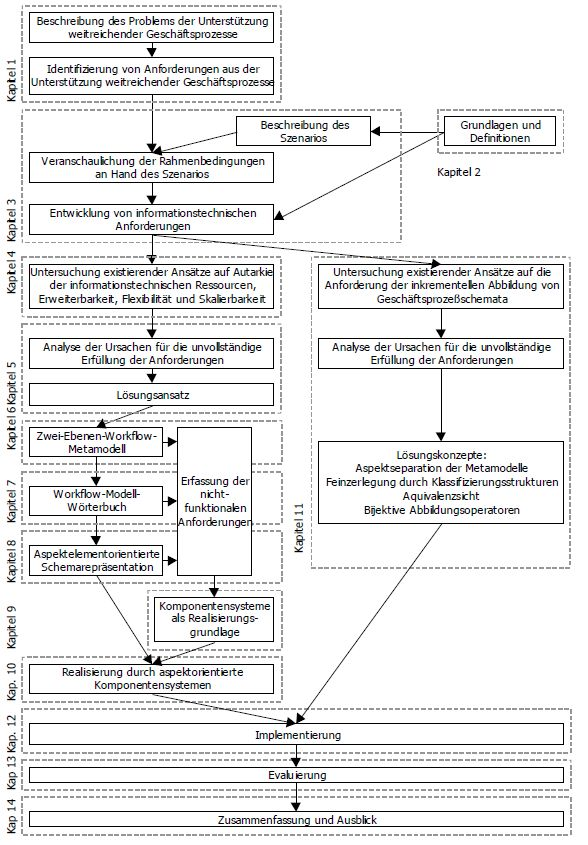
\includegraphics[height=0.9\textheight]{images/ausarbeitung.jpg}
  \caption{vorgehen nach \autocite{Schmidt:Geschaeftsprozesse}}
  \label{fig:1}
\end{figure}


% ---
\chapter{Grundlagen}
\label{cha:grundlagen}

In diesem Kapitel das für das Praktikum relevante Grundlagenwissen 
dargestellt. Der Praktikant soll hierzu das ihm durch Vorlesungen 
bekannte, bzw. durch Recherchen vertiefte theoretische Wissen 
darstellen, das für die Lösung der im Praktikum gestellten Probleme 
notwendig ist.

Dabei ist darauf zu achten, nur solche Inhalte in das Grundlagenkapitel 
aufzunehmen, die später auch verwendet werden (Problembezogenheit). 
Ebenso ist auf eine ausreichend tiefe und vollständige Darstellung der 
Grundlagen zu achten.

Für die Erstellung des Literaturverzeichnisses 
wird das Werkzeug JabRef\autocite{JabRef:JabRef} verwendet. 

Sie können aber auch das Werkzeug Citavi\autocite{SAS:Citavi} benutzen
und dort nach \textsc{Bib}\TeX{} exportieren.

\section{Grundlagengebiet A}
\label{sec:grundlagengebieta}

\subsection{Definition AA}
\label{sub:definitionaa}

\subsection{Definition AB}
\label{sub:definitionab}

\section{Grundlagengebiet B}
\label{sec:grundlagengebietb}

\subsection{Definition BA}
\label{sub:definitionBa}

\subsection{Definition BB}
\label{sub:definitionbb}

%---
\chapter{Problemanalyse}
\label{cha:problemanalyse}

Die Analyse des zu lösenden Problems ist Grundlage für jedes 
ingenieurmäßige Vorgehen. Daher soll in diesem Kapitel das zu lösenden 
Problem auf Basis des im Grundlagenkapitel aufbereiteten Wissens 
analysiert werden. Hierzu ist insbesondere notwendig zu klären, wie sich 
das Gesamtproblem in Teilprobleme zerlegen lässt und welche 
Abhängigkeiten zwischen diesen bestehen.

Bei Software-Projekten befindet sich an dieser Stelle typischerweise die 
Anforderungsanalyse des \ac{rup}.

%---
\chapter{Typen und Objekte}
\label{cha:types_and_objects}

\section{Definition von Typen}
\label{sec:types}
Analog zu klassischen Klassen (oder Strukturen) in C++ muss ein offener Typ vor Benutzung, d.h. Erzeugung von Objekten dieses Typen, erst definiert werden. 
Zuerst muss dafür ein Typ, hier als Beispiel der Typ \textit{Person}, mit
\mint{cpp}|OT_TYPE(Person)|
definiert werden.
Dies erzeugt intern zwei Klassen/Strukturen:
\begin{itemize}
\item \mint{cpp}|struct ot_types::Person : public ot::Type|
\item \mint{cpp}|struct Person : public ot::Reference<ot_types::Person>|
\end{itemize}
\textit{ot{\_}types::Person} ist hierbei die interne Repräsentation des Typen und für den Benutzer offener Typen nicht direkt relevant. Sie erbt von
der Basisklasse für alle offene Typen \textit{ot::Type}.
Die für den Benutzer wichtige Klasse \textit{Person} erweitert den internen Typen um die Referenzsemantik.

\section{Referenzsemantik}
\label{sub:objects_references}
Um die aus anderen Hochsprachen, zum Beispiel Java oder C{\#}, gewohnte Referenzsemantik auch für die offenen Typen zu ermöglichen erbt die, durch die Definition eines Typen entstehende, Klasse \textit{Person} von 
\mint{cpp}|public ot::Reference<ot_types::Person>|
\textit{ot::Reference<T>} ist für die Speicherverwaltung und für boolesche Vergleichsoperatoren zuständig. \textit{ot::Reference<T>} besitzt hierzu einen Zeiger auf den Typ T 
\mint{cpp}|T* ptr = nullptr;| 
Die booleschen Vergleichsoperatoren werden durch klassische Vergleiche auf Zeiger abgebildet. D.h zwei Referenzen sind gleich, wenn sie auf den gleichen Speicherbereich zeigen und eine Referenz kann implizit nach \textit{bool} mit \textit{ptr != nullptr} umgewandelt werden. Die Speicherverwaltung wird durch Referenzzählung implementiert. Um zu gewährleisten, dass der Speicherbereich erst freigegeben wird, wenn ihn keine Referenz mehr referenziert, ist die Referenzzählung in die Singleton-Klasse
\mint{cpp}|class PtrManager| 
ausgelagert. Diese zählt die Referenzierungen für jeden Speicherbereich und bietet Methoden um die jeweilige Anzahl zu inkrementieren bzw. zu dekrementieren. Eine Referenz inkrementiert den Zähler, wenn sie mit einem Zeiger initialisiert wird. Sie dekrementiert den Zähler im Destruktor. Wenn die Referenz den Zeiger einer anderen Referenz kopiert, wird erst der Zähler für den aktuellen Zeiger dekrementiert und dann der Zähler für den kopierten Zeiger inkrementiert. Wenn nach einer Dekrementierung der Zähler gleich 0 ist, wird der Speicherbereich des Zeigers freigegeben. Für einen Zeiger auf \textit{nullptr} wird die Inkrementierung/Dekrementierung übersprungen.

\section{Erzeugen von Objekten}
\label{sec:objects}
Mit dem Typen \textit{Person} können nun, wie in C++ üblich, Objekte erzeugt werden
\mint{cpp}|Person person;| 

\subsection{Nil-Objekte}
\label{sub:objects_nil}
Standardmäßig ist ein Objekt eines Typen ein Nil-Objekt, d.h. die Referenz referenziert \textit{nullptr}. Dies kann auch explizit mit
\mint{cpp}|Person person = Person::nil();|
geschrieben werden. Auch beim Testen, ob ein Objekt ein Nil-Objekt ist, kann der explizite Aufruf auf \textit{Person::nil} verwendet werden.
\mint{cpp}|if (person == Person::nil()) { /*...*/ }| 
ist hierbei gleich bedeutend wie 
\mint{cpp}|if (!person) { /*...*/ }| 

\subsection{Leere Objekte}
\label{sub:objects_empty}
Um ein tatsächliches Objekt des Typen zu erzeugen muss dieses über die statische \textit{create}-Methode des Typen
\mint{cpp}|person = Person::create();| 
erzeugt werden. Eine andere Referenz kann nun diese Referenz kopieren
\mint{cpp}|Person person2 = person;| 

%---
\chapter{Attribute}
\label{cha:attributes}
Um einem Typen ein ein- oder mehrwertiges Attribut zu geben, muss dafür der Attributname, der Typ und der Datentyp des Attributs angegeben werden
\mint{cpp}|OT_ATTR1(name, Person, std::string)|
bzw.
\mint{cpp}|OT_ATTRN(tags, Person, std::string)|
Die Attribute an sich sind als Funktionen mit dem Attributsnamen als Funktionsname implementiert. Für jede Zugriffsweise auf ein Attribut (Lesen, Schreiben, Löschen etc.) gibt es (mindestens) eine Funktion mit jeweils unterschiedlicher Parameterliste.

\section{Einwertige Attribute}
\label{sec:attributes_1}
Einwertige Attribute sind die einfachste Form eines Attributes. Entweder hat das Attribut einen Wert, oder nicht.

\subsection{Lesen}
\label{sub:attributes_1_read}
Es gibt zwei Arten ein Attribut zu lesen:
\begin{itemize}
\item \mint{cpp}|std::string name = person[name];|
\item \mint{cpp}|std::string name = name(person);|
\end{itemize}
Der überladene \textit{[]}-Operator des Typen, ruft dann im Endeffekt für \textit{person[name]} wiederrum intern \textit{name(person)} auf. Wenn das Attribut nicht gesetzt wurde, wird der Standardwert des Attributdatentyps zurückgegeben. Im diesem Fall wäre das \textit{std::string()} oder \textit{"{}"{}}(leerer String).

\subsection{Schreiben}
\label{sub:attributes_1_write}
Um ein Attribut zu setzen bzw. zu überschreiben:
\begin{itemize}
\item \mint{cpp}|person(name, std::string("Hans"));|
\item \mint{cpp}|name(person, std::string("Hans"));|
\end{itemize}
Da ein string-Literal in C++ den Typ \textit{const char*} hat, muss hier zwingend die explizite Umwandlung in einen \textit{std::string} beim Setzen des Attributs passieren. Alternativ kann auch direkt ein Wert vom Typ \textit{std::string} übergeben werden
\begin {minted}{cpp}
std::string value = "Peter";
person(name, value);
\end{minted}

\subsection{Löschen}
\label{sub:attributes_1_remove}
\begin{itemize}
\item \mint{cpp}|person -= name;|
\item \mint{cpp}|name(person, ot::DeleteDefault{});|
\end{itemize}
Da sich die Parameterliste für jede Funktion mit dem gleichen Funktionsnamen unterscheiden muss, das Löschen eines (einwertigen) Attributes aber eigentlich keine zusätzlichen Parameter außer dem Objekt (wie beim lesenden Zugriff) braucht, muss hier beim Löschen über den Attributnamen noch ein Objekt des Typs \textit{ot::DeleteDefault} übergeben werden.

\section{Mehrwertige Attribute}
\label{sec:attributes_N}

\subsection{ot::vector}
\label{sub:attributes_N_ot_vector}

\subsection{Lesen der Attributliste}
\label{sub:attributes_N_read}

\subsection{Hinzufügen eines Attributwerts am Ende der Liste}
\label{sub:attributes_N_write_end}

\subsection{Hinzufügen eines Attributwerts an einer bestimmten Position der Liste}
\label{sub:attributes_N_write_index}

\subsection{Löschen der gesamten Attributliste}
\label{sub:attributes_N_remove}

\subsection{Löschen eines bestimmten Attributwerts aus der Liste}
\label{sub:attributes_N_remove_value}

\subsection{Löschen eines Attributwerts an einer bestimmten Position aus der Liste}
\label{sub:attributes_N_remove_index}

%---
\chapter{Bidirektionale Relationen}
\label{cha:relations}

\section{Asymmetrische Relationen}
\label{sec:relations_asymmetric}

\subsection{1:1-Relationen}
\label{sub:relations_asymmetric_1_1}

\subsection{1:N-/N:1-Relationen}
\label{sub:relations_asymmetric_1_N}

\subsection{N:N-Relationen}
\label{sub:relations_asymmetric_N_N}

\section{Symmetrische Relationen}
\label{sec:relations_symmetric}

\subsection{1:1-Relationen}
\label{sub:relations_symmetric_1_1}

\subsection{N:N-Relationen}
\label{sub:relations_symmetric_N_N}

%---
\chapter{Typen und Attribute als Schablonen}
\label{cha:templates}

\section{Typschablonen}
\label{sec:templates_types}

\section{Einwertige Attribute für Typschablonen}
\label{sec:templates_attributes_1}

\section{Mehrwertige Attribute für Typschablonen}
\label{sec:templates_attributes_N}

%---
\chapter{Namensbereiche}
\label{cha:objects_namespaces}

%---
\chapter{Serialisierung und Deserialisierung mit cereal}
\label{cha:templates}

\section{cereal}
\label{sec:cereal}

\section{Serialisierung eines Typen}
\label{sec:cereal_save}

\section{Deserialisierung eines Typen}
\label{sec:cereal_save}

%---
\chapter{Evaluierung}

Aufgabe des Kapitels Evaluierung ist es, in wie weit die Ziele der 
Arbeit erreicht wurden. Es sollen also die erreichten Arbeitsergebnisse 
mit den Zielen verglichen werden. Ergebnis der Evaluierung kann auch 
sein, das bestimmte Ziele nicht erreicht werden konnten, wobei die 
Ursachen hierfür auch außerhalb des Verantwortungsbereichs des 
Praktikanten liegen können.

%---
\chapter{Zusammenfassung und Ausblick}
\label{cha:zusammenfassung}

\section{Erreichte Ergebnisse}
\label{sec:ergebnisse}

Die Zusammenfassung dient dazu, die wesentlichen Ergebnisse des 
Praktikums und vor allem die entwickelte Problemlösung und den 
erreichten Fortschritt darzustellen. (Sie haben Ihr Ziel erreicht und 
dies nachgewiesen).

\section{Ausblick}
\label{sec:ausblick}

Im Ausblick werden Ideen für die Weiterentwicklung der erstellten Lösung 
aufgezeigt. Der Ausblick sollte daher zeigen, dass die Ergebnisse der 
Arbeit nicht nur für die in der Arbeit identifizierten Problemstellungen 
verwendbar sind, sondern darüber hinaus erweitert sowie auf andere 
Probleme übertragen werden können.

\subsection{Erweiterbarkeit der Ergebnisse}
\label{sub:erweiterbarkeit}

\subsection{Übertragbarkeit der Ergebnisse}
\label{sub:uebertragbarkeit}

%-----------------------------------------------------------------------
\appendix

%---
\printbibliography

%---
\chapter{Anhang A}

%---
\chapter{Anhang B}


\end{document}